% Minimal phase/offset probe for patterns.meta Lines.
\usetikzlibrary{patterns.meta}

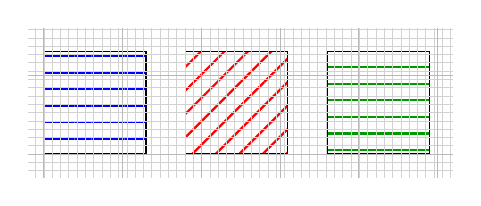
\begin{tikzpicture}[x=1cm,y=1cm]
  % Baseline problematic case (horizontal blue).
  \path[draw,pattern={Lines[distance=6pt,line width=.8pt]},pattern color=blue] (0,0) rectangle +(1.3,1.3);

  % Same spacing with angle to verify phase/origin under rotation.
  \path[draw,pattern={Lines[distance=6pt,line width=.8pt,angle=45]},pattern color=red] (1.8,0) rectangle +(1.3,1.3);

  % Same spacing with shifts to ensure x/y phase offsets are preserved.
  \path[draw,pattern={Lines[distance=6pt,line width=.8pt,xshift=1pt,yshift=2pt]},pattern color=green!60!black] (3.6,0) rectangle +(1.3,1.3);

  % Overlay reference grid for easier phase/offset comparison.
  \draw[step=3pt,gray!35,line width=.1pt] (-0.2,-0.3) grid (5.2,1.6);
  \draw[step=1cm,gray!55,line width=.16pt] (-0.2,-0.3) grid (5.2,1.6);
\end{tikzpicture}
